\documentclass[8pt, letterpaper, titlepage]{article}
\usepackage[utf8]{inputenc}
\usepackage{geometry}
\usepackage{color,graphicx,overpic} 
\usepackage{fancyhdr}
\usepackage{amsmath,amsthm,amsfonts,amssymb}
\usepackage{mathtools}
\usepackage{hyperref}
\usepackage{multicol}
\usepackage{array}
\usepackage{float}
\usepackage{blindtext}
\usepackage{longtable}
\usepackage{scrextend}
\usepackage[font=small,labelfont=bf]{caption}
\usepackage[framemethod=tikz]{mdframed}
\usepackage{calc}
\usepackage{titlesec}
\usepackage{listings}
\usepackage[normalem]{ulem}
\usepackage{tabularx}
\usepackage{mathrsfs}
\usepackage{bookmark}
\usepackage{setspace}
\usepackage{tabularx}
\usepackage{ltablex}
\usepackage{enumitem}
\usepackage[simplified]{pgf
-umlcd}
\definecolor{dkgreen}{rgb}{0,0.6,0}
\definecolor{gray}{rgb}{0.5,0.5,0.5}
\definecolor{mauve}{rgb}{0.58,0,0.82}
\usepackage{listings}

\lstset{frame=tb,
  language=Java,
  aboveskip=3mm,
  belowskip=3mm,
  showstringspaces=false,
  columns=flexible,
  basicstyle={\small\ttfamily},
  numbers=none,
  numberstyle=\tiny\color{gray},
  keywordstyle=\color{blue},
  commentstyle=\color{dkgreen},
  stringstyle=\color{mauve},
  breaklines=false,
  breakatwhitespace=true,
  tabsize=3
}

\mathtoolsset{showonlyrefs}  
\allowdisplaybreaks

\definecolor{mycolor}{rgb}{0, 0, 0}

\geometry{top=2.54cm, left=2.54cm, right=2.54cm, bottom=2.54cm}

% Indentation/space between paragraphs
\setlength{\headheight}{15pt}
\setlength{\parindent}{0pt}
\setlength{\parskip}{0pt}

% Line spacing
\renewcommand{\baselinestretch}{1.5} 

% Line spacing
\renewcommand{\baselinestretch}{1.3} 

% Title page
\title{\textbf{\Huge{ 
\begin{center}
MATE 201\\ \large{Class notes} % Document name
\end{center} 
}}}

\author{Lora Ma}

% Header/Footer
\pagestyle{fancy}
\fancyhf{}
\rhead{\thepage}
\lhead{\textit{CMPUT 366 - A2}}
\rfoot{}

% Hyperlink colors
\hypersetup{
    colorlinks=true,
    linkcolor=blue,
    filecolor=blue,      
    urlcolor=blue,
}

\begin{document}

\section*{Analyzing the Scatter Plot}
\begin{figure}[H]
  \begin{center}    
    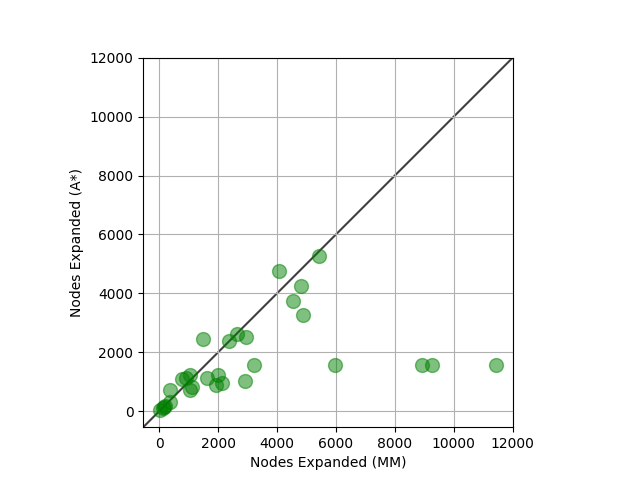
\includegraphics[width=\linewidth*3/6]{image.png}
    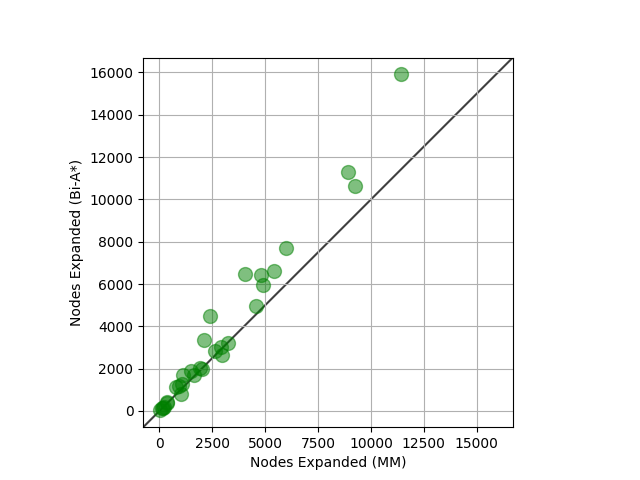
\includegraphics[width=\linewidth*3/6]{image1.png}
  \end{center}
\end{figure}
\begin{enumerate}
  \item Decrease
  \item D. If A* expands 27\% fewer states than Dijkstra's algorithm, then A* will be about 27\% faster than Dijkstra's algorithm. This is because most of the run time is occupied by expansions; however A* will be a bit less than 27\% faster than Dijkstra's algorithm because of overhead costs such as initializing the open and closed lists. 
  \item As shown in the second graph above, MM tends to perform fewer expansions than Bi-A*
  \item No, in general the number of expansions were quite similar
  \item In the first plot above, most of the points where a solution was found had similar number of expansions; however there are a few outliers where no solution is found and there are more nodes expanded using MM than A*. MM tries to balance expanding nodes in the forward and backwards lists, so it takes longer before the algorithm finds out there is no solution whereas A* expands in one direction until it discovers there is no solution
\end{enumerate}
\end{document}